\documentclass[a4paper,11pt]{article}

\newcommand{\XX}{\textbf{XX}\xspace}
\newcommand{\TheProject}{\XX}

\usepackage{lscape} % for landscape
\usepackage{comments}
% %\usepackage[final]{comments}
\usepackage{verbatim}
\usepackage{listings}
\usepackage{supertabular,array}
\makeatletter
\newcommand\arraybslash{\let\\\@arraycr}
\makeatother
% \setlength\tabcolsep{1mm}
% \renewcommand\arraystretch{1.3}
%% Related Projects
\newcommand{\scienceproject}{\mbox{\textsc{SCIEnce}}}
\newcommand{\OOMMFNB}{OOMMF-NB}

\newcommand{\software}[1]{\texttt{#1}\xspace}
\newcommand{\GAP}{\software{GAP}}
\newcommand{\libGAP}{\software{libGAP}}
\newcommand{\Singular}{\software{Singular}}
\newcommand{\Sage}{\software{Sage}}
\newcommand{\SageCombinat}{\software{Sage-Combinat}}
\newcommand{\MuPADCombinat}{\software{MuPAD-Combinat}}
\newcommand{\Sphinx}{\software{Sphinx}}
\newcommand{\Python}{\software{Python}}
\newcommand{\IPython}{\software{IPython}}
\newcommand{\Jupyter}{\software{Jupyter}}
\newcommand{\Cython}{\software{Cython}}
\newcommand{\Pythran}{\software{Pythran}}
\newcommand{\Numpy}{\software{Numpy}}
\newcommand{\Pari}{\software{PARI}}
\newcommand{\PariGP}{\software{PARI/GP}}
\newcommand{\Linbox}{\software{LinBox}}
\newcommand{\LMFDB}{\software{LMFDB}}
\newcommand{\OpenEdX}{\software{OpenEdX}}
\newcommand{\Linux}{\software{Linux}}
\newcommand{\LATEX}{\software{\LaTeX}}
\newcommand{\SMC}{\software{SageMathCloud}}
\newcommand{\Simulagora}{\software{Simulagora}}
\newcommand{\Magma}{\software{Magma}}
\newcommand{\Mathematica}{\software{Mathematica}}
\newcommand{\Maple}{\software{Maple}}
\newcommand{\Matlab}{\software{Matlab}}
\newcommand{\MPIR}{\software{MPIR}}
\newcommand{\Arxiv}{\software{arXiv}}

%%% Local Variables: 
%%% mode: latex
%%% TeX-master: "proposal"
%%% End: 

% Partners
\newparticipant{PS}{Université Paris Sud}{UPS}{FR}
\newparticipant{LL}{Logilab}{Logilab}{FR}
\newparticipant{UV}{Université de Versailles Saint-Quentin}{UVSQ}{FR}
\newparticipant{UJF}{Université Joseph Fourier}{UJF}{FR}
\newparticipant{UB}{Université Bordeaux}{UB}{FR}
\newparticipant{UO}{University of Oxford}{UO}{UK}
\newparticipant{USH}{Université of Sheffield}{USHEF}{UK}
\newparticipant{USO}{Université of Southampton}{USO}{UK}
\newparticipant{SA}{University of St Andrews}{USTAN}{UK}
\newparticipant{UW}{University of Warwick}{UW}{UK}
\newparticipant{JU}{Jacobs University Bremen}{JU}{DE}
\newparticipant{UK}{University of Kaiserslautern}{UK}{DE}
\newparticipant{US}{University of Silesia}{US}{PL}
\newparticipant{ZH}{Universit\"{a}t Z\"{u}rich}{UZH}{CH}
\newparticipant{SR}{Simula Research Laboratory}{Simula}{NO}
\newparticipant{UWS}{University of Washington at Seattle}{UWS}{US}
% Participant or third party?
% Jean-Pierre Flori
% Luca DeFeo
% Jean-Guillaume Dumas
% Clément Pernet

% Personalised comments for each author
\newcommand{\slcomment}[1]{\comment{SL}{#1}}
\newcommand{\akcomment}[1]{\comment{AK}{#1}}

%% Related Projects
\newcommand{\scienceproject}{\mbox{\textsc{SCIEnce}}}


%%% Local Variables: 
%%% mode: plain-tex
%%% TeX-master: "proposal"
%%% End: 


\begin{document}

\begin{titlepage}

\begin{center}
{\Large \textbf{COVER PAGE}}
\end{center}

\begin{tabular}{llr}
\textbf{Title of Proposal:} & \textbf{\TheProject{}: Collaborative ecosystems for mathematical research and software development} & \\[2ex] % \includeimage[scale=0.5]{logo} \\
\textbf{Date of preparation:} & \textbf{\today} & \comment{}{$
$Revision: 0.0$ $}\\[2ex]
\textbf{List of participants} && \\[2ex]


\end{tabular}

\begin{center}
\begin{tabular}{|l|p{3in}|l|l|}\hline
Participant no & Participant organisation name & Country\\

\hline
1 (Coordinator) & \longparticipant{1} & \country{1}  \\ \hline
2 & \longparticipant{2} & \country{2}  \\ \hline
3 & \longparticipant{3} & \country{3}  \\ \hline
4 & \longparticipant{4} & \country{4}  \\ \hline
5 & \longparticipant{5} & \country{5}  \\ \hline
6 & \longparticipant{6} & \country{6}  \\ \hline
7 & \longparticipant{7} & \country{7}  \\ \hline
\end{tabular}
\end{center}

\tableofcontents

\eucommentary{Please follow the structure of this template when
  preparing your proposal. It has been designed to ensure that the
  important aspects of your planned work are presented in a way that
  will enable the experts to make an effective assessment against the
  evaluation criteria. Sections 1, 2 and 3 each correspond to an
  evaluation criterion for a full proposal.\\
  Please be aware that proposals will be evaluated as they were
  submitted, rather than on their potential if certain changes were to
  be made. This means that only proposals that successfully address
  all the required aspects will have a chance of being funded. There
  will be no possibility for significant changes to content, budget
  and consortium composition during grant preparation.\\
  Page limit: The cover page, and sections 1, 2 and 3, together should
  not be longer than 70 pages. All tables in these sections must be
  included within this limit. The minimum font size allowed is 11
  points. The page size is A4, and all margins (top, bottom, left,
  right) should be at least 15 mm (not including any footers or
  headers).  If you attempt to upload a proposal longer than the
  specified limit, before the deadline you will receive an automatic
  warning, and will be advised to shorten and re-upload the
  proposal. After the deadline, any excess pages will be overprinted
  with a ‘watermark’, indicating to evaluators that these pages must
  be disregarded.\\
  Please do not consider the page limit as a target! It is in your
  interest to keep your text as concise as possible, since experts
  rarely view unnecessarily long proposals in a positive light.}
\end{titlepage}

\newpage

\begin{draft}
\red

\section*{Outline of Project (for Proposers)}

\TODO{This is the place for various READMEs not included in the final submission}

\subsection*{Vision}

An internal attempt at specifying our vision through short
(unsubstantiated) answers.

\begin{verbatim}
> 1) Who are we?

Lead or core developers of some of the major open source components
for pure mathematics and applications:

- Computational components: GAP, Linbox, MPIR, Pari, Sage, Singular
- Databases: LMFDB (findstat as well)
- Knowledge management: MathHub

Together with, in a larger scientific domain, lead developers for:

- Collaborative user interfaces (IPython, SageMathCloud)
- Database and Scientific Computing for the industry (Logilab)
- Numerical code optimization/parallelisation (Pythran)

> 2) What is our goal?

Building blocks with a sustainable development model that can be
seamlessly combined together to build versatile high performance
VRE's, each tailored to a specific need in pure mathematics and
application.

> 2.5) What is our strategy?

Maximize sustainability and impact by reusing and improving existing
building blocks, and reaching toward larger communities whenever possible.
E.g. factoring out our common user interface needs at the level
of IPython/Jupyter will save us time (sustainability), and impact
the larger scientific computing community.
The improvements to the building blocks will impact all their users,
whether they use the VRE or not.

> 3) From where do we start?

- Building blocks with a sustainable development model
- Proof-of-concept prototypes of VRE (SMC, Simulagora)
- Experience on combining together some of the building blocks

> 4) How do we connect or differ from other projects?

The other projects focus on either one or a few of the building
blocks, or on a specific VRE.

We articulate our work with each of them.

> 5) Why are we excellent?

The consortium puts together recognized experts in all
areas and most building blocks that are relevant to the goal. There is
simultaneously a variety of point of views and a record of past
experiences collaborating together at smaller scale
(e.g. GAP-Singular). The approach is bottom up.  Most joint tasks
consist in bringing together people with a common need. There is
experience in community building.  Most participants are
simultaneously users and developers of their tools.

All of this makes me confident that we will indeed be able to
productively collaborate. And do stuff that is first class and useful.

On Sat, Dec 13, 2014 at 11:18:10PM +0100, Wolfram Decker wrote:
> 0) What precisely is our starting point and why are we the right people to
> achieve what we promise to do? Are we leaders in the area touched
> by the proposal? How do we connect? Is there some past
> collaborative success?
> 1) You still do not say what we actually will provide. What precisely will
> the VRE offer to its users?

I more or less answered those points above. Let me know if I should
elaborate.

> Who will be its users? Will those already familiar with the involved
> CAS use it? Will it make the CAS more attractive for a much larger
> community?

One objective is definitely to make CAS and others more attractive by
lowering a lot the entry barrier to access the soft (and db, ...). A
typical situation that most of us ran into is, when collaborating with
other less tech-savvy mathematicians, to have trouble sharing code,
data, and in-the-writing papers with them. SMC was launched with this
idea in mind, and the success proves the concept.

At the same time, the improvements in the building blocks will also
impact CAS users that are happy with their current user interface /
work-flow.

Improvements to IPython will impact a much larger community.

> 2) You motivate what we wish to do by the success of SageMathCloud.
> But why do we than need another VRE? How do we differ from
> SageMathCloud?

There is no one-size-fits-all VRE. One might want to run a VRE on
one's own computer resources for a variety of reason (speed of access,
specific resources, privacy, independence, ...). One might want a
different combination of software (e.g. a lightweight VRE with only
Singular).  One might want to focus on data with LMFDB-style database
searches, or on interactive computing, or on document writing, or some
combination thereof.

> Do we have a chance to compete? Or will we rather join forces? In
> which way?

We join forces (the plan is to have William/UW in the consortium, as
non funded participant). SMC focuses on one specific cloud based
VRE. We focus on the building blocks and the glue. Both project are
mutually beneficial. See the language p. 14 of the proposal.

> 3) You motivate what we wish to do by the success of LMFDB. But what
> are our connections to this database? Will we enhance it? Will we connect
> it to other stuff we do? Will we create other databases?

LMFDB is a prototype of large scale database. We want to make it
easier for other groups of mathematicians to setup similar databases
in their area. Reciprocally, like SMC, the LMFDB with benefit back
from the improved building blocks.

> 4) Why is Europe in the lead if there is already SageMathCloud?
> Where precisely is Europe in the lead?

Europe is the lead in many of the building blocks.
\end{verbatim}

% \subsection*{Mission statement for the grant}

% Our mission is to promote the next generation of community-developed
% open source software, databases, and services adapted to the needs of
% collaborative research in pure mathematics and applications.

% Our research will cover a wide variety of aspects, ranging from
% software development models, user interfaces \TODO{virtual
%   environments?}, deployment frameworks and novel collaborative tools,
% component architecture, design, and standardization of software
% \TODO{system?} and databases, to links to publication, data archival
% and reproducibility of experiments, development models and tools, and
% social aspects.

% It will consolidate Europe's leading position in computational
% mathematics and build on the remarkable success of the ecosystem of
% projects GAP, Python/Sage, Pari, Singular, LMFDB.

\subsection*{Description of the call}

\verbatiminput{call_description}

% \TODO{What do we mean by ``new generation''}.

\renewcommand{\thepage}{\arabic{page}}
\setcounter{page}{1}
\black
\cleardoublepage
\end{draft}

%%% Local Variables: 
%%% mode: latex
%%% TeX-master: "proposal"
%%% End: 


% ---------------------------------------------------------------------------
%  Section 1: Excellence
% ---------------------------------------------------------------------------

\section{Excellence}

\subsection{Objectives}
\label{sect:objectives}

\eucommentary{\emph{Describe the specific objectives for the project,
which should be clear, measurable, realistic and achievable within the
duration of the project. Objectives should be consistent with the expected
exploitation and impact of the project (see section 2).}}

\TODO{The pieces of material below need to be recombined in a flowing
  story.}

\subsubsection{Key ideas}:
\begin{itemize}
\item Experimental maths has become a core asset for research in pure
  mathematics and its applications.
\item Over the last decades, mathematicians have gained strong
  experience in collaborative software development, with pioneering
  work and continuing leadership of Europe.
\item Mathematicians have a strong tradition of sharing knowledge
  openly (arxiv, Wikipedia, ...).
\item Mathematicians have been building and sharing databases for a
  long while; the needs for such is growing tremendously, and the
  process needs to be streamlined.
\end{itemize}


This project gathers European core developers of leading mathematical
software (GAP, Pari, Sage, Singular, ...), databases (LMFDB, ...), and
critical components (IPython stack), together with researchers in
computer and social sciences, with mission to promote a new generation
of community-developed open source software \TODO{more precisely
  what's new is the combination thereof!}, databases, and services,
adapted to the needs of collaborative research in pure mathematics and
its applications.

\TODO{Keyword: flexible virtual environment}

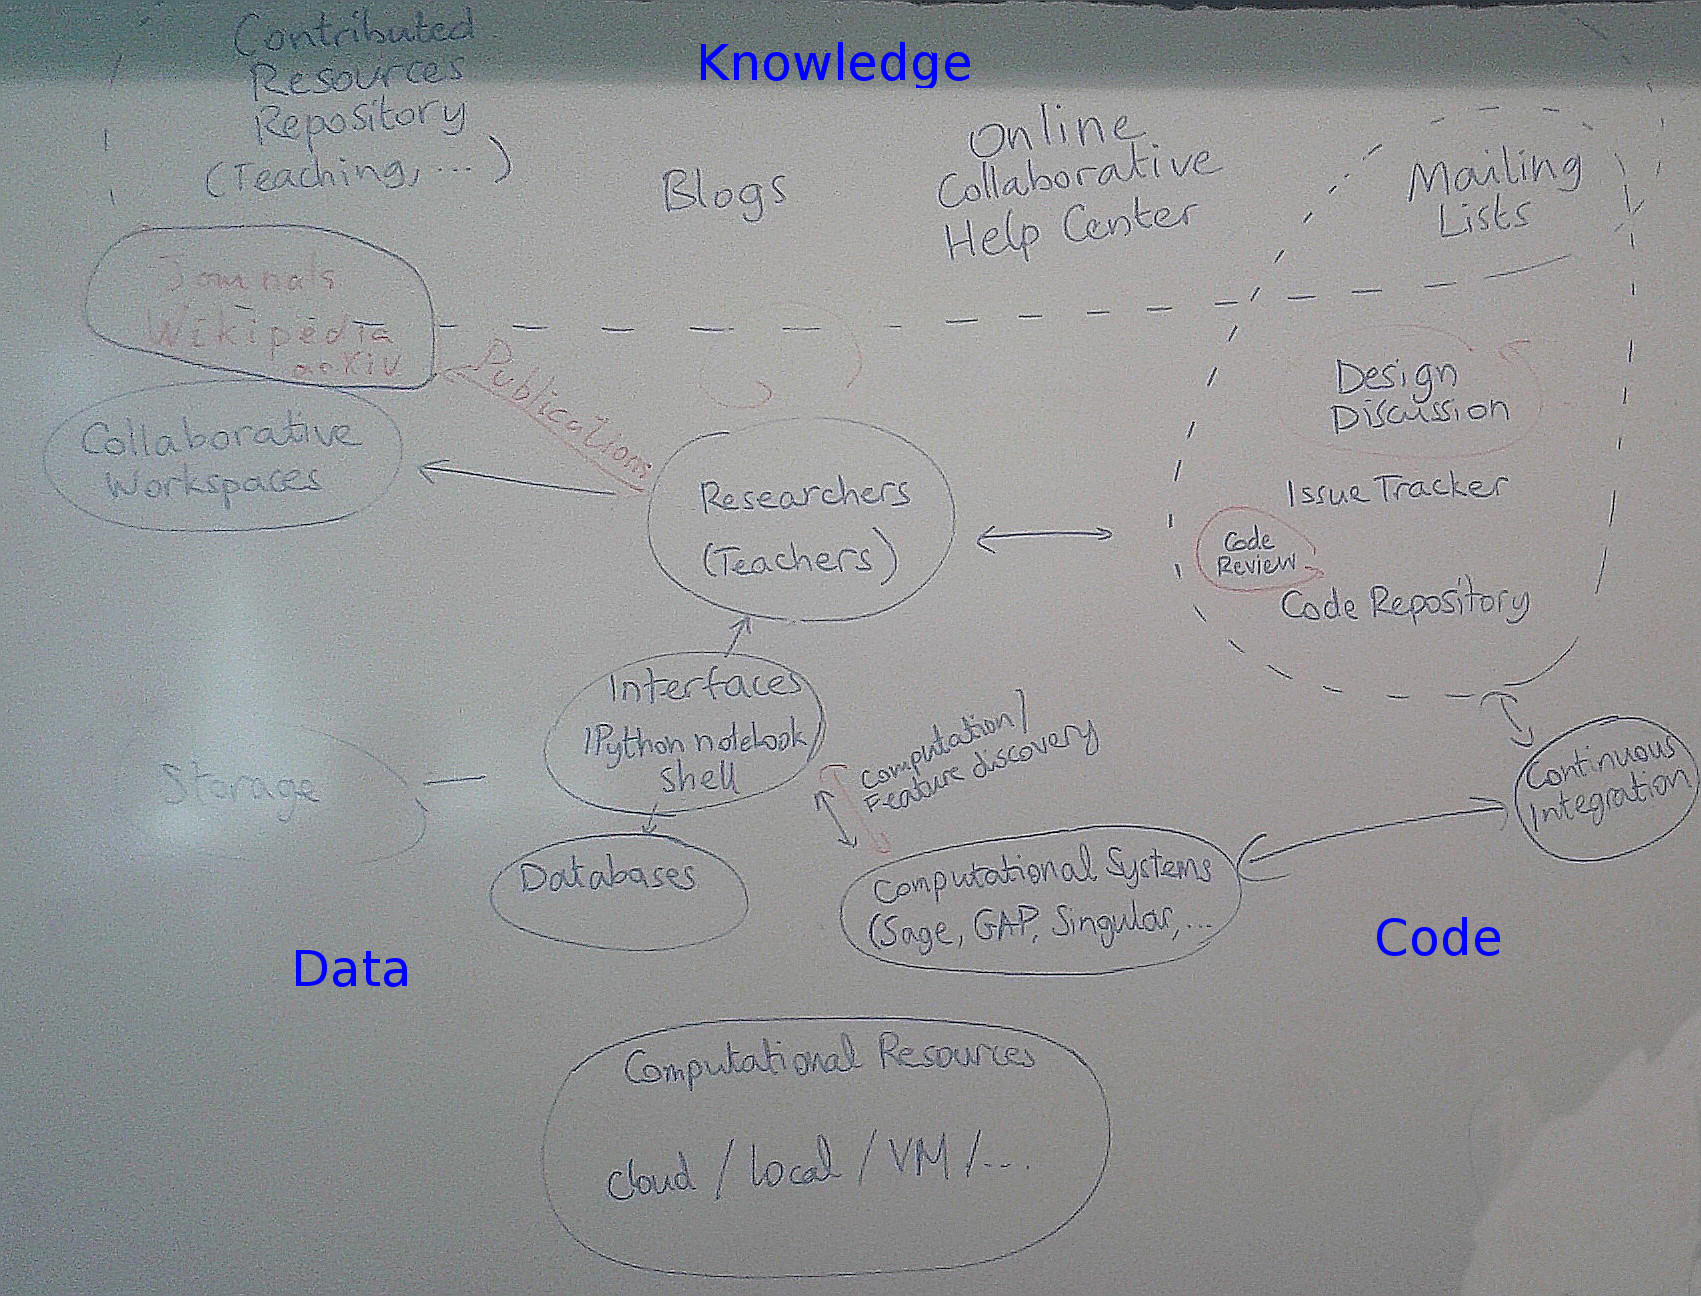
\includegraphics{Pictures/TheBigPicture.jpg}

Our research will cover a wide variety of aspects, ranging from
software development models, user interfaces \TODO{virtual
  environments?}  deployment frameworks and novel collaborative tools,
component architecture, design, and standardization of software
components and databases, to links to publication, data archival and
reproducibility of experiments, development models and tools, and
social aspects. It will build on the remarkable success of the open
source ecosystem and consolidate Europe's leading position in
computational mathematics.

\subsubsection{Why collaborative development of open source software?}

From their early days, computers have been used in pure mathematics,
either to prove theorems or, like the telescope for astronomers, to
explore new theories. Major achievements include the proof of the four
color theorem or \TODO{Nice flashy example?}. Usage has grown to the
point that certain areas of mathematics now completely depend on
experimental methods, with major efforts spent on software
development. As the sophistication of the required computations
increased, supported by the boom of the available computational power,
it became vital to share those efforts at the scale of large research
communities. European mathematicians have been pioneers and have grown
a steady tradition of collaborative open source software development,
with systems like GAP, Singular, or Pari/GP playing a major role for
decades.

\subsubsection{Importance of experimental tools in maths}

The field of computer algebra allows us to compute in and with a multitude
of mathematical structures. It is interdisciplinary in nature, with links to quite
a number of areas in mathematics, with applications in mathematics and other
branches of science and engineering, and with constantly new and often
surprising developments. Quite a number of these developments, in fact the
creation of whole subareas of the field,  have been iniated by European
researchers who made crucial contributions at all levels. These include the
design of fundamental algorithms, the development of major computer
algebra systems, applications of the computational methods in various fields,
and the creation of widely used data bases.

Particular fruitful interactions unfold between computer algebra and
algebraic geometry, number theory, and group theory. Algebraic algorithms
open up new ways of accessing subareas of these key disciplines of
mathematics, and they are fundamental to practical applications of the
disciplines. Conversely, challenges arising in algebraic geometry, number
theory, and group theory quite often lead to algorithmic breakthroughs
which, in turn, open the door for new theoretical and practical applications
of computer algebra.

Based on exact computer aided calculations, the experimental method has
now been added to the toolbox of the pure mathematician. Experiments
lead to new conjectures which may have a deep impact on the future
development of mathematics. An outstanding example is the Birch and
Swinnerton-Dyer conjecture which is one of the Clay Millenium Problems.
Data bases relying on computer calculations such as the Small Groups
Library or the Modular Atlas in group and representation theory provide
indispensible tools for researchers. A constructive way of understanding
proofs of deep theorems yields algorithmic tools to deal with highly abstract
concepts. These tools make the concepts available to a broader class of
researchers, with many potential applications. A prominent example from
algebraic geometry is the desingularization theorem of Hironaka, for which
Hironaka won the fields medal, and its algorithmization by Villamayor.

Spectacular theoretical breakthrougs such as Wiles' proof of Fermat's last
theorem are based on interdisciplinary approaches. Current developments
on the algorithmic side allow one to conquer crossconnections between
different areas of mathematics also computationally and, thus, to
arrive at cutting-edge applications which previously were inconceivable.





\draftpage

\subsection{Relation to the Work Programme}

\eucommentary{
Indicate the work programme topic to which your proposal relates, and
explain how your proposal addresses the specific challenge and scope
of that topic, as set out in the work programme.}

\eucommentary{
  \verbatiminput{call_description}
}

\draftpage

\subsection{Concept and Approach}

\eucommentary{
-- Describe and explain the overall concept underpinning the project.
Describe the main ideas, models or assumptions involved. Identify
any trans-disciplinary considerations;}

\eucommentary{Describe any national or international research and innovation activities which will be
linked with the project, especially where the outputs from these will feed into the
project;}

\begin{itemize}
\item DFG Priority Project SPP 1489: \url{computeralgebra.de}
  \TOWRITE{WD}{}
  (in particular already may joint activities; see ...)
\item IPython grant
\item FLINT grant
\item Sage-Combinat grant
\end{itemize}

\eucommentary{
-- Describe and explain the overall approach and methodology, distinguishing, as
appropriate, activities indicated in the relevant section of the work programme, e.g.
Networking Activities, Service Activities and Joint Research Activities, as detailed in
the Part E of the Specific features for Research Infrastructures of the Horizon 2020
European Research Infrastructures (including e-Infrastructures) Work Programme 2014-
2015;\\
-- Describe how the Networking Activities will foster a culture of co-operation between the
participants and other relevant stakeholders.\\
-- Describe how the Service activities will offer access to state-of-the-art infrastructures,
high quality services, and will enable users to conduct excellent research.\\
-- Describe how the Joint Research Activities will contribute to quantitative and qualitative
improvements of the services provided by the infrastructures.\\
-- As per Part E of the Work Programme, where relevant, describe how the project will
share and use existing basic operations services (e.g. authorisation and accounting
systems, service registry, etc.) with other e-infrastructure providers and justify why such
services should be (re)developed if they already exist in other e-infrastructures. Describe
how the developed services will be discoverable on-line.\\
-- Where relevant, describe how sex and/or gender analysis is taken into account in the
project�s content.}

\draftpage

\subsection{Ambition}

\eucommentary{-- Describe the advance your proposal would provide beyond the
state-of-the-art, and the extent the proposed work is ambitious. Your answer
could refer to the ground-breaking nature of the objectives, concepts
involved, issues and problems to be addressed, and approaches and methods to be used.\\
-- Describe the innovation potential which the proposal represents. Where relevant, refer to
products and services already available, e.g. in existing e-Infrastructures.}

\draftpage

% ---------------------------------------------------------------------------
%  Section 2: Impact
% ---------------------------------------------------------------------------

\section{Impact}
\label{sec:impact}

\subsection{Expected Impacts}

\eucommentary{Please be specific, and provide only information that applies
to the proposal and its objectives. Wherever possible, use quantified
indicators and targets.\\
Describe how your project will contribute to:\\
-- the expected impacts set out in the work programme, under the relevant topic
(including key performance indicators/metrics for monitoring results and impacts);\\
-- improving innovation capacity and the integration of new knowledge
(strengthening the competitiveness and growth of companies by developing
innovations meeting the needs of European and global markets; and, where
relevant, by delivering such innovations to the markets;\\
-- any other environmental and socially important impacts (if not already
covered above).\\
Describe any barriers/obstacles, and any framework conditions (such as
regulation and standards), that may determine whether and to what extent
the expected impacts will be achieved. (This should not include any risk
factors concerning implementation, as covered in section 3.2.)}

\draftpage

\subsection{Measures to Maximise Impact}

\subsubsection{Dissemination and Exploitation of Results}
\label{subsubsect:dissemination}

\eucommentary{-- Provide a draft 'plan for the dissemination and exploitation
of the project's results'. The plan, which should be proportionate to the
scale of the project, should contain measures to be implemented both during
and after the project.\\
Dissemination and exploitation measures should address the full range
of potential users and uses including research, commercial, investment,
social, environmental, policy making, setting standards, skills and
educational training.\\
The approach to innovation should be as comprehensive as possible,
and must be tailored to the specific technical, market and organisational
issues to be addressed\\
-- Explain how the proposed measures will help to achieve the expected impact of the
project . Provide a draft business plan for financial sustainability as stated in the Part
E of the Specific features for Research Infrastructures of the Horizon 2020 European
Research Infrastructures (including e-Infrastructures) Work Programme 2014-2015.\\
-- Where relevant, include information on how the participants will
manage the research data generated and/or collected during the
project, in particular addressing the following issues:
What types of data will the project generate/collect? What
standards will be used? How will this data be exploited and/or
shared/made accessible for verification and re-use (If data cannot
be made available, explain why)? How will this data be curated and preserved?\\ \\
-- Include information about any open source software used or developed by the
project.\\
You will need an appropriate consortium agreement to manage (amongst other things)
the ownership and access to key knowledge (IPR, data etc.). Where relevant,
these will allow you, collectively and individually, to pursue market opportunities
arising from the project's results.\\
The appropriate structure of the consortium to support exploitation is addressed
in section 3.3. \\ \\
-- Outline the strategy for knowledge management and protection. Include measures to
provide open access (free on-line access, such as the �green� or �gold� model) to
peer-reviewed scientific publications which might result from the project.\\
Open access publishing (also called 'gold' open access) means that an article is
immediately provided in open access mode by the scientific publisher. The associated costs
are usually shifted away from readers, and instead (for example) to the university or
research institute to which the researcher is affiliated, or to the funding agency supporting
the research.\\
Self-archiving (also called 'green' open access) means that the published article or the
final peer-reviewed manuscript is archived by the researcher - or a representative - in an
online repository before, after or alongside its publication. Access to this article is often -
but not necessarily - delayed (�embargo period�), as some scientific publishers may wish to
recoup their investment by selling subscriptions and charging pay-per-download/view fees
during an exclusivity period.}

\draftpage

\subsubsection{Communication activities}
\label{subsubsect:communication}

\eucommentary{Describe the proposed communication measures for promoting the
project and its findings during the period of the grant. Where appropriate
these measures should include social media and public events with user
participation. Measures should be proportionate to the scale of the project,
with clear objectives. They should be tailored to the needs of various audiences,
including groups beyond the project's own community. Where relevant, include
measures for public/societal engagement on issues related to the project.}

\clearpage

% ---------------------------------------------------------------------------
%  Section 3: Implementation
% ---------------------------------------------------------------------------



\section{Implementation}

\subsection{Work Plan --- Work packages, deliverables and milestones}
\label{sect:workplan}

\eucommentary{Please provide the following:\\
\begin{itemize}
\item
brief presentation of the overall structure of the work plan;
\item
timing of the different work packages and their components (Gantt chart or similar);
\item
detailed work description, i.e.:
\begin{itemize}
\item
a description of each work package (table 3.1a);
\item
a list of work packages (table 3.1b);
\item
a list of major deliverables (table 3.1c);
\end{itemize}
\item
graphical presentation of the components showing how they inter-relate (Pert chart or similar).
\end{itemize}
}

\subsubsection*{Overall Structure of the Work Plan}

The work plan is broken down into XX workpackages as shown
in Figure~\ref{}: WP2 deals with  ...
In addition, there is one management work package (WP1) and one
general dissemination work package (\ref{m}). The Gantt chart on
Page~\pageref{fig:gantt} illustrates the timeline for the
various tasks for these work packages, including inter-task
dependencies.

%\newpage
\subsubsection*{How the Work Packages will Achieve the Project Objectives}
\label{sssec:how_the_work_packages_will_achieve}

\TOWRITE{ALL}{This needs to explain that we're actually going to meet the
objectives.  Needs to be done after objectives and WPs.}

The project objectives (Section~\ref{sect:objectives},
page~\pageref{sect:objectives}) and the corresponding work
packages that contribute to achieving those objectives are:

\begin{center}
\begin{tabular}{|l|l|l|}\hline
\textbf{Objective} & \textbf{Purpose} & \textbf{WPs} \\\hline \hline
Objective 1 & XX & \textbf{WPX} \\\hline
\end{tabular}
\end{center}

\paragraph*{Work Programme for Objective 1: }

Objective 1 is covered by WPX, which will ...

\landscape

\subsubsection*{Work Plan Timing: GANTT Chart showing Task Dependencies and Information Flows}


\vspace{-0.7in} \centerline{\hbox to \columnwidth{\hss%\includeimage[scale=0.85,angle=270]{ParaPhrase-Gantt2.pdf}
\hss}}
\label{fig:gantt}
\vspace{-1in} % Fool LaTeX into avoiding unnecessary page break
\endlandscape

\newpage

%\input{deliverables-dates}
%% Deliverables list.
%% Deliverables ordered by Workpackage
%% Workpackages are numbered automatically in sequence - the WP number has no effect

\workpackage{1}{Project Management}
\deliverable{mgt:mailinglists}
\deliverable{mgt:projectwebsite}
\deliverable{mgt:swrepository}
\deliverable{mgt:periodic-rep-1}
\deliverable{mgt:periodic-rep-2}
\deliverable{mgt:periodic-rep-3}
\deliverable{mgt:periodic-rep-4}
\deliverable{mgt:final-mgt-rep}
% Metrics: in PM and a bit in each work package

\workpackage{2}{Community Building and Engagement}
\deliverable{del:xx}

\workpackage{3}{Component Architecture}
\deliverable{del:xx}

%\workpackage{XXX}{Standardization} % => Component architecture + advertisement in the dissemination
%\deliverable{del:xx}

\workpackage{4}{User Interfaces}
\deliverable{del:xx}

\workpackage{5}{HPC and massively parallel components}
\deliverable{del:xx}

\workpackage{6}{Next generation Mathematical Databases}
\deliverable{del:xx}
%SL

\workpackage{7}{Development Models for an Academic Free Software Ecosystem}
\deliverable{del:xx}
%SL? Dima?

\workpackage{8}{Social Aspects}
\deliverable{del:xx}
%UM
%\workpackage{XXX}{Supporting the Mathematical Process} % => A chunk of Social Aspects
%\deliverable{del:xx}


\workpackage{9}{Dissemination, Exploitation and Communication}
\deliverable{del:pressrelease} % Press release.
\deliverable{del:website} % Project presentation (web site). 
\deliverable{del:workshop1}  % Report on first project workshop, year 1. 
\deliverable{del:dissemplan1} % Final plan for using and disseminating knowledge.
\deliverable{del:workshop2}  % Report on second project workshop, year 2
\deliverable{del:workshop3}  % Report on third project workshop, year 3
\deliverable{del:dissemplan2} % Final plan for using and disseminating knowledge.


\addtocounter{subsubsection}{1}
\addcontentsline{toc}{subsubsection}{\protect\numberline{\thesubsubsection}Work
Package List}
\fbox{\begin{minipage}{\textwidth}\begin{center}{\Large\bf
        Work package list} % (full duration of project)}
  \end{center}
  \end{minipage}}

\bigskip\bigskip

\begin{tabular}{|p{1.2cm}|p{9.15cm}|p{0.8cm}|p{1.2cm}|p{1cm}|p{0.9cm}|p{0.9cm}|}
\hline
{\bf Work \mbox{package} No} & {\bf Work package title} &
{\bf Lead \mbox{partic.} no.} &
{\bf Lead short name} &
{\bf Person months} & {\bf Start month} & {\bf End month} \\\hline

\newcounter{wp}

\addtocounter{wp}{1}
\workpackageentry{\thewp}{SA}{}{1}{60}

\addtocounter{wp}{1}
\workpackageentry{\thewp}{}{}{}{}

\addtocounter{wp}{1}
\workpackageentry{\thewp}{}{}{}{}

\addtocounter{wp}{1}
\workpackageentry{\thewp}{}{}{}{}

\addtocounter{wp}{1}
\workpackageentry{\thewp}{}{}{}{}

\addtocounter{wp}{1}
\workpackageentry{\thewp}{}{}{}{}

\addtocounter{wp}{1}
\workpackageentry{\thewp}{}{}{}{}

\addtocounter{wp}{1}
\workpackageentry{\thewp}{}{}{}{}

\addtocounter{wp}{1}
\workpackageentry{\thewp}{SA}{}{}{}

{\textbf{Total}} & & & &
\textbf{\large XXX}&
&
\\\hline
\end{tabular}


% \textbf{Summary:}\\[1ex]

\newpage

\fbox{\begin{minipage}{\textwidth}\begin{center}\Large\bf List of Deliverables
  \end{center}
  \end{minipage}}

\label{sect:deliverables}

\bigskip\bigskip\bigskip

\begin{minipage}{\textwidth}
\begin{center}
\begin{tabular}{|p{0.8cm}|p{8.75cm}|p{0.8cm}|p{1.2cm}|p{1.2cm}|p{1.2cm}|p{1.2cm}|}  \hline
\textbf{Del. no.}              & \textbf{Deliverable name}        & \textbf{WP no.} & \textbf{Lead}
& \textbf{Type}              & \textbf{Dissemi- nation level}   & \textbf{Delivery date}
\\ \hline

%% Year 1

\ref{del:xx}  & Requirements Analysis
& WP? & & R & CO &  ?? \\
\hline
\end{tabular}
\end{center}
\end{minipage}


\newpage

%% Set up the milestone numbers.
\eucommentary{Milestones means control points in the project that help to chart progress. Milestones may
correspond to the completion of a key deliverable, allowing the next phase of the work to begin.
They may also be needed at intermediary points so that, if problems have arisen, corrective
measures can be taken. A milestone may be a critical decision point in the project where, for
example, the consortium must decide which of several technologies to adopt for further
development.}

The work in the \TheProject project is structured by four milestones,
which coincide with the four project meetings held at the end of each
year of the project (the other four meetings will be held in the middle
of each year). Given the nature of the project, with a
large number of essentially independent tasks, there is no need for
milestones attached to specific collections of tasks or
deliverables. Instead, given that the meetings are the main
face-to-face interaction points in the project, it's suitable to
schedule the milestones for these events, where they can be discussed
in detail, tracking the progress in each work package through status
reports on the tasks and deliverables.

We envisage that this setup will give the project the vital coherence
in spite of the broad interdisciplinary mix of various backgrounds of the
participants.

% \newcommand{\WPall}{\WPref{management}, \WPref{dissem}, \WPref{component-architecture}, \WPref{UI}, \WPref{hpc}, \WPref{dksbases}, \WPref{social-aspects}}

% \newcommand{\WPnoUI}{\WPref{management}, \WPref{dissem}, \WPref{component-architecture}, \WPref{hpc}, \WPref{dksbases}, \WPref{social-aspects}}

% \begin{center}
%   \begin{tabular}{|m{.05\textwidth}|m{.30\textwidth}|m{.15\textwidth}|m{.05\textwidth}|m{.22\textwidth}|}
%     \hline
%     Mile-stone nr. & Milestone name & Related work packages & Est. date & Means of verification \\\hline
%     M1 & Requirements study, design and prototype implementations. Start of
%          community building.
%        & \WPall 
%        & 12 
%        & 2nd Project meeting report. Completion of corresponding deliverables. \\\hline
%     M2 & First fully functional interface implementations.
%          Enhanced versions of \TheProject components.
%          Training early adopters.
%        & \WPall 
%        & 24 
%        & 4th Project meeting report. Completion of corresponding deliverables. \\\hline
%     M3 & Evaluating \TheProject software. Working with the community 
%          and building portfolio of experiments produced with \TheProject.
%        & \WPall 
%        & 36 
%        & 6th Project meeting report. Completion of corresponding deliverables. \\\hline
%     M4 & Project evaluation and final versions of all \TheProject components.
%        & \WPnoUI 
%        & 48 
%        & 8th Project meeting report. Completion of corresponding deliverables. \\\hline
%   \end{tabular}
% \end{center}

\begin{milestones}
  \milestone[id=startup,month=12,
  verif={Completed all corresponding deliverables and reported the progress in the 2nd Project meeting report.}]
  {Startup}
  {By Milestone 1 we will have carried out the requirements study, design and prototype implementations and started community building activities.}

  \milestone[id=proto1,month=24,
  verif={Completed all corresponding deliverables and reported the progress in the 4th Project meeting report.}]
  {Prototypes}
  {By Milestone 2 we will have constructed first fully functional interface implementations and released enhanced versions of \TheProject components, and train early adopters of \TheProject.}

  \milestone[id=community,month=36,
  verif={Completed all corresponding deliverables and reported the progress in the 6th Project meeting report.}]
  {Community/ Experiments}
  {By Milestone 3 we will have gathered and evaluated feedback on \TheProject software and established the portfolio of experiments produced with \TheProject through further engaging with the community.}

  \milestone[id=eval,month=48,
  verif={Completed all corresponding deliverables and reported the progress in the 8th Project meeting report.}]
  {Evaluation}
  {By Milestone 4 we will have released final versions of all \TheProject components and completed the project evaluation.}
\end{milestones}

%%% Local Variables:
%%% mode: latex
%%% TeX-master: "proposal"
%%% End:

%  LocalWords:  verif ldots


\fbox{\begin{minipage}{\textwidth}\begin{center}\Large\bf List of milestones
  \end{center}
  \end{minipage}}
\label{sect:milestones}

\bigskip\bigskip\bigskip

\begin{minipage}{\textwidth}
\begin{center}
\begin{tabular*}{\textwidth}{|p{1.5cm}|p{6.7cm}|p{2.5cm}|p{1.5cm}|p{3.6cm}|}  \hline
\textbf{Milestone number} & \textbf{Milestone name} & \textbf{Related work
  package(s)} & \textbf{Estimated date} & \textbf{Means of
  verification} (deliverables shown here + success criteria below) \\
\hline
\ref{mil:initial} &
  Completed initial requirements analysis.  &
  WPX &
  1 &
\ref{del:requirements-analysis}.
\\
\ref{mil:final} &
&
WPX &
&
\\
\hline
\end{tabular*}
\end{center}
\end{minipage}

\vspace{10pt}
\begin{center}
\begin{tabular*}{\textwidth}{|p{1.5cm}|p{13.3cm}|p{1.9cm}|}\hline
\textbf{Milestone} & \textbf{Success Criteria} & \textbf{Contributes to
  Objective(s)} \\\hline
\ref{mil:initial} &
Completed requirements analysis (Deliverable~\ref{del:requirements-analysis}). &
 \textbf{1, 3.}
\\
\ref{mil:final} &
XX
& \textbf{XX}
\\\hline
\end{tabular*}
\end{center}


% ---------------------------------------------------------------------------
% Include Workpackage descriptions
% ---------------------------------------------------------------------------

%% WP titles and order are defined in deliverables.tex
%%% Workpackage style may be broken -- fix this!!

%% Local WP number counter - should possibly be global and hidden?

\newcounter{wpno}

\addtocounter{wpno}{1}

\begin{Workpackage}{\thewpno}
\WPTitle{\wpname{\thewpno}}
\WPStart{Month 1}
\WPParticipant{SA}{60}

\begin{WPObjectives}
The objectives of \theWP{} are to undertake all project management activities, including ...

\end{WPObjectives}

\begin{WPDescription}
This workpackage will perform ...
\end{WPDescription}

\begin{WPDeliverables}
\begin{itemize}
\item
\ref{mgt:mailinglists}
(Month 1): 
Internal and external mailing lists.
\item
\ref{mgt:swrepository}
(Month 1): 
Internal software repository.
\item
\ref{mgt:periodic-rep-1}
(Month 12): 
Project Periodic Report (first year).
\item
\ref{mgt:periodic-rep-2}
 (Month 24): 
Project Periodic Report (second year).
\item
\ref{mgt:periodic-rep-3}
(Month 36): 
Project Periodic Report (third year).
\item
\ref{mgt:periodic-rep-4}
(Month 48): 
Project Periodic Report (fourth year).
\item
\ref{mgt:final-mgt-rep}
(Month 36): 
Project Final Report
\end{itemize}
\end{WPDeliverables}
\end{Workpackage}

\addtocounter{wpno}{1}
\begin{Workpackage}{\thewpno}
\wplabel{wp:x}
\WPTitle{\wpname{\thewpno}}
\WPStart{Month 1}
\WPParticipant{SA}{1}

\begin{WPObjectives}
The objectives of \theWP{} are to:
\begin{itemize}
\item
\item
\item
\item
\item
\end{itemize}
\end{WPObjectives}

\begin{WPDescription}
This workpackage  ...
\end{WPDescription}

\begin{WPDeliverables}
\begin{itemize}
\item
\ref{del:x}
(Month X): 
X.
\end{itemize}
\end{WPDeliverables}
\end{Workpackage}

\addtocounter{wpno}{1}
\begin{Workpackage}{\thewpno}
\wplabel{wp:x}
\WPTitle{\wpname{\thewpno}}
\WPStart{Month 1}
\WPParticipant{SA}{1}

\begin{WPObjectives}
The objectives of \theWP{} are to:
\begin{itemize}
\item
\item
\item
\item
\item
\end{itemize}
\end{WPObjectives}

\begin{WPDescription}
This workpackage  ...
\end{WPDescription}

\begin{WPDeliverables}
\begin{itemize}
\item
\ref{del:x}
(Month X): 
X.
\end{itemize}
\end{WPDeliverables}
\end{Workpackage}

\endinput

\input{WPs/WP4}
\input{WPs/WP5}
\input{WPs/WP6}
\input{WPs/WP7}
\input{WPs/WP8}
\input{WPs/WP9}
\input{WPs/WP10}
\input{WPs/WP11}
\input{WPs/WP12}
\input{WPs/WP13}
\input{WPs/WP14}
\input{WPs/WP15}


\TODO{Milestones need to be discussed and then described here.}

\newpage

\TODO{Check this for any necessary changes.}


\subsection{Management Structure and Procedures}
\label{sect:mgt}

\eucommentary{Describe the organisational structure and the decision-making
(including a list of milestones (table 3.2a)).\\
Explain why the organisational structure and decision-making mechanisms are
 appropriate to the complexity and scale of the project.\\
Describe, where relevant, how effective innovation management will be
addressed in the management structure and work plan.\\
Describe any critical risks, relating to project implementation, that
the stated project's objectives may not be achieved. Detail any risk
mitigation measures. Please provide a table with critical risks
identified and mitigating actions (table 3.2b).}

\draftpage
\subsection{Consortium as a Whole}
\eucommentary{\begin{itemize}
\item
Describe the consortium. How will it match the project's objectives?
How do the members complement one another (and cover the value chain,
where appropriate)? In what way does each of them contribute to the
project? How will they be able to work effectively together?
\item
If applicable, describe the industrial/commercial involvement in the
project to ensure exploitation of the results and explain why this is
consistent with and will help to achieve the specific measures which
are proposed for exploitation of the results of the project (see section 2.3).
\item
Other countries: If one or more of the participants requesting EU funding
is based in a country that is not automatically eligible for such funding
(entities from Member States of the EU, from Associated Countries and
from one of the countries in the exhaustive list included in General
Annex A of the work programme are automatically eligible for EU funding),
 explain why the participation of the entity in question is essential to carrying out the project
\end{itemize}
}

\TODO{Select some events from the list on \url{computeralgebra.de} to
  highlight the existing tight collaborations between the members.}

\TODO{Explanation of why we want to include Seattle (sage-math cloud,
  is a key component; access to IP).}

\draftpage

\subsection{Resources to be Committed}

\eucommentary{Please provide the following:
\begin{itemize}
\item
a table showing number of person/months required (table 3.4a)
\item
a table showing 'other direct costs' (table 3.4b) for participants where
those costs exceed 15\% of the personnel costs (according to the budget
table in section 3 of the administrative proposal forms)
\end{itemize}}

\TOWRITE{ALL}{Proofread 3.4 pass 2 (especially first paragraph Staff efforts)}

\eucommentary{Please provide the following:
\begin{compactitem}
\item
a table showing number of person/months required (table 3.4a)
\item
a table showing 'other direct costs' (table 3.4b) for participants where
those costs exceed 15\% of the personnel costs (according to the budget
table in section 3 of the administrative proposal forms)
\end{compactitem}}

\subsubsection{Management Level Description of Resources and Budget}
\label{sect:budget-details}

\paragraph{Staff efforts}

\eucommentary{Please indicate the number of person/months over the whole
duration of the planned work, for each work package, for each participant.
Identify the work-package leader for each WP by showing the relevant
person-month figure in bold.}

By design \TheProject is attacking upfront the diverse needs of a
very large community: pure maths and applications. Thanks to its
toolkit approach, it will impact users in many areas of science. This
is a major long term investment which requires the extensive expertise
of a large consortium and the improvement of a great number of
software components. The complex technical nature of the project,
combined with the high quality requirements for guaranteeing long term
sustainability, necessitates recruiting highly experienced software
engineers to complement the participants. Much emphasis is put as well
on studying the social aspects and implementing many demonstrators to
illustrate the breath and depth of potential applications.

This all explains the considerable staff efforts%
\ifgrantagreement.\else %
displayed in the following table.
\wpfig[label=fig:staffeffort,caption=Summary of Staff Efforts]
\fi

\paragraph{Travel, dissemination, and outreach}

The community-building nature of this grant proposal requires a large
number of staff exchanges, workshops with project partners, as well as
workshops engaging the wider community in addition to the usual
management and project review meetings. For dissemination, we need to
target the computer science and computational science-focused
communities and their conferences, as well as the domains benefitting
from \TheProject, such as Mathematics and Physical Sciences.

\subparagraph{Guidelines for travel and dissemination}
\label{sect:budget-details-travel}

We use the following guidelines for expected travel expenses:
\euro{2200} for attendance of a typical one week international
conference outside Europe (including travel, subsistence,
accommodation and registration), \euro{1200} for a corresponding
conference in Europe, \euro{750} for a one-week visit of a  project
partner, for instance for coding sprints and one-to-one 
research visits. We expect a similar cost per week while hosting
visitors. For the half-yearly project meetings, we expect on average a
cost of \euro{400} for travel, accommodation and subsistence.

For a partner site with one investigator and one full time researcher,
we expect that that both will attend all of the 9 project meetings that take
place every 6 months (cost of 9 * 2 * 400 =
\euro{7200}), and that the site spends \euro{2000} per year to host
external visitors contributing to the project (total \euro{8000}). We
expect the investigator and the researcher in total to do 4 one-week visits
to other sites (each at \euro{750}) every year, totaling \euro{12000} over 4 years).

% 9*2*400 + 2000*4 + 4*750*4
For dissemination, we expect the researcher to attend on average 1
international conference and 2 European meetings per year (totals
\euro{18400}) and the investigator to attend one international and one
european gathering (totals \euro{13600}).
% (2*2200 + 3*1200)*4

Where there are multiple investigators per site, they will share the
travel and associated costs outlined above. Where there are multiple
researchers, or researchers not employed for the full 48 months, the
travel budget is reduced accordingly.

\subparagraph{Guidelines for outreach costs}
\label{sect:budget-outreach-publication-charges}
We also request \euro{1000} per year per partner (several partners
have other means do pay these costs, and for them these are not needed) 
to pay for open access publication charges.

\label{sect:budget-outreach-workshops}
We request funds for outreach activities such as workshops that
facilitate community building, disseminate best practice and
encourages sustained contributions of the community to the project and
beyond the lifetime of the funding. For  a one-week workshop reaching
out to the community, we cost these at about 400 EUR per participant
to provide accommodation and catering. A workshop for 15 people will
thus cost about \euro{6000}. Participants donate their time and will fund
their own travel. The particular budgeted cost will depend on the
local availability of accommodation and will thus vary from workshop to
workshop. We use creative means to increase value and improve
community building where possible, for example by cooking food
ourselves as done in this recent workshop
\href{http://wiki.sagemath.org/days57}{http://wiki.sagemath.org/days57}.

Details are given in the tables below and in the work packages.

\bigskip

\subsubsection{Resource summaries for consortium member sites}
\label{resources.summary}

%%%%%%%%%%%%%%%%%%%%%%%%%%%%%%%%%%%%%%%%%%%%%%%%%%%%%%%%%%%%%%%%
%
% Guidelines for completion of partner specific resource summary:
%
%
% Please explain how many person months for each person are
% requested. Say who is the local lead. Say anything that helps to
% understand why people are recruited as you plan, in particular if
% this deviates from having one research for 48 months.  We can also
% use this bit of the proposal (and the table, see below) to address
% any other unusual arrangements.
%
%
% The table should contain all non-staff costs (the EU requests that
% this table must be present if the non-staff costs exceed
% 15% of the total cost, but it is good practice and will show
% openness and transparency that we show the data for all partners).
%
% Link back from the table to the work packages and tasks for which
% the expenses are required. Add information that makes it easier to
% understand why the expenses are justified.
%
%     To refer to a task in a work package, use "\taskref{WP-ID}{TASK-ID}" where
%     WP-ID is the ID of the work package:
%        WP#: WP-ID - full title
%        ----------------------
%        WP1: 'management' - Management
%        WP2: 'community' - Community Building and Engagement
%        WP3: 'component-architecture' - Component Architecture
%        WP4: 'UI' - User interfaces
%        WP5: 'hpc' - High Performance Computing
%        WP6: 'dksbases' - Data/Knowledge/Software-Bases
%        WP7: 'social-aspects' - Social Aspects
%        WP8: 'dissem' - Dissemination
%
%
%     and "TASK-ID" is the ID of the task. You can set this using
%
%       \begin{task}[id=TASK-ID,title=Math Search Engine,lead=JU,PM=10,lead=JU]
%
%     To refer to deliverables, use "\delivref{WP-ID}{DELIV-ID}" where DELIV-ID is
%     the ID of the deliverable that can be set like this:
%
%       \begin{wpdeliv}[due=36,id=DELIV-ID,dissem=PU,nature=DEM]
%           {Exploratory support for semantic-aware interactive widgets providing views on objects
%           represented and or in databases}
%       \end{wpdeliv}
%
%
% The table is pre-populated with entries most sites are likely
% to need. If a line does not apply to you, just delete it. If you need
% an extra line, then add it. Use common sense: the number of rows should not
% be very big, but at the same time it is useful to give some breakdown/explanation
% of costs.
%
%
% Eventually, try to create you entry similar in style to the others.
% (The Southampton entry is fully populated, so use this as guidance
% if in doubt.)
%
%
%%%%%%%%%%%%%%%%%%%%%%%%%%%%%%%%%%%%%%%%%%%%%%%%%%%%%%%%%%%%%%%%

In this section we briefly describe the requested resources. See the
participant descriptions in the description of the consortium for the
specific role of each member.

%%%%%%%%%%%%%%%%%%%%%%%%%%%%%%%%%%%%%%%%%%%%%%%%%%%%%%%%%%%%%%%%%%%%%%%%%%%%%%
\paragraph{Resources Université Paris-Sud}

\site{PS} requests 12 person months for the project coordinator
(Nicolas M. Thiéry), 5 person months for two researchers (Florent
Hivert, and Samuel Lelièvre) and for the lead PI (Viviane Pons), 48+36
months for two full time developers, 36 months for a PhD student, and
24 months for a part time project manager for the full duration of the
project.

% 4 * 4k: Developper workshops Cernay
% 6k: Jupyter-Sage
% 2 * 6k: Women in Sage
% Training: 2*4k
% Dissemination CIRM: 16k
% Kickup and final meeting: 2*16k
% workshop: 82k
% (2 * 4 + 3 + 2 * 4 )*(1*2200 + 2*1200) + 2*2000 + 4*750
% travel: 103K


% update table as is appropriate for your contribution. Please remove unused lines.
\bigskip
\begin{table}[H]
\begin{tabular}{|r|r|p{8.5cm}|}
\hline
\textbf{1: \site{PS}} & \textbf{Cost (\euro)} & \textbf{Justification} \\\hline
\textbf{Travel} & 103,000 & Travel (see the guidelines \ref{sect:budget-details-travel})\\\hline
\textbf{Publication charges} & 1,000 & Open access publication charges (see \ref{sect:budget-outreach-publication-charges})\\\hline
%\textbf{Equipment} & ?,??? &  \\\hline    %\taskref{WP-ID}{TASK-ID}
\textbf{Other goods and services} & 92,000 & 8 developer
workshops~\taskref{dissem}{devel-workshops}, 4 training and
dissemination workshops~\taskref{dissem}{dissemination-communication},
audits certificates on the financial statements \\\hline   %\taskref{WP-ID}{TASK-ID} \delivref{WP-ID}{DELIV-ID}
\textbf{Total} & 196,000\\\cline{1-2}
\end{tabular}
\caption{Overview: Non-staff resources to be committed at \site{PS} (all in \texteuro)}\vspace*{-1em}
\end{table}

%%%%%%%%%%%%%%%%%%%%%%%%%%%%%%%%%%%%%%%%%%%%%%%%%%%%%%%%%%%%%%%%%%%%%%%%%%%%%%
\paragraph{Resources CNRS}

CNRS requests 12 person months for the lead PI Vincent Delecroix and
the \PariGP head Karim Belabas, 6 person months for PIs
Bill Allombert and Adrien Boussicault, 5 person months for PI Loïc Gouarin, and
48 person months for a full time developer working on tasks~\taskref{hpc}{hpc-pari},
\taskref{hpc}{hpc-combi}, \taskref{UI}{Sage-display} and \taskref{UI}{pari-python}.

\bigskip
\begin{table}[H]
\begin{tabular}{|r|r|p{8.5cm}|}
\hline
\textbf{2: \site{UB}} & \textbf{Cost (\euro)} & \textbf{Justification} \\\hline
\textbf{Travel}
  &  56,700 & Travel (see the guidelines \ref{sect:budget-details-travel})\\\hline
\textbf{Publication charges}
  &   1,000 & Open access publication charges (see \ref{sect:budget-outreach-publication-charges})\\\hline
%%\textbf{Equipment}
%%  &   0 &  \\\hline    %\taskref{WP-ID}{TASK-ID}
\textbf{Other goods and services}
  & 111,000 &
1 HPC workshop \taskref{dissem}{devel-workshops},
4 Ateliers \Pari \taskref{dissem}{devel-workshops},
4 dissemination workshop in developing countries \taskref{dissem}{dissemination}
 \\\hline   %\taskref{WP-ID}{TASK-ID} \delivref{WP-ID}{DELIV-ID}
\textbf{Total}
 & 168,700\\\cline{1-2}
\end{tabular}
\caption{Overview: Non-staff resources to be committed at \site{CNRS} (all in \texteuro)}\vspace*{-1em}
\end{table}


%%%%%%%%%%%%%%%%%%%%%%%%%%%%%%%%%%%%%%%%%%%%%%%%%%%%%%%%%%%%%%%%%%%%%%%%%%%%%%
\paragraph{Resources Jacobs University Bremen}

\site{JU} requests 6 PM each for the PIs (Prof. Michael Kohlhase leads \WPref{dksbases})
and Dr. habil Florian Rabe (theoretical foundations of triform theories). Furthermore, we
request 24 PM each for a research programmer (Dr. Christian Maeder) and a junior
researcher (Mihnea Iancu M.Sc.). The first will do much of the actually system development
in \WPref{UI} and \WPref{dksbases} while the latter will concentrate on the cases studies
in \WPref{dksbases}.

\bigskip
\begin{table}[H]
\begin{tabular}{|r|r|p{8.5cm}|}
  \hline
  \textbf{3: \site{JU}} & \textbf{Cost (\euro)} & \textbf{Justification} \\\hline
  \textbf{Travel} & 53,600 & Travel (see the guidelines \ref{sect:budget-details-travel})\\\hline
  \textbf{Publication charges} & 4,000 & Open access publication charges (see \ref{sect:budget-outreach-publication-charges})\\\hline
  \textbf{Equipment} & 14,000 &  for two web/compute servers for~\taskref{UI}{mathhub};
   they need 256 GB RAM each for the math search engine from~\taskref{dksbases}{mws}\\\hline
\textbf{Other goods and services} & 4,300 & Audits certificates on the financial statements \\\hline
\textbf{Total} & 75,900\\\cline{1-2}
\end{tabular}
\caption{Overview: Non-staff resources to be committed at \site{JU} (all in \texteuro)}\vspace*{-1em}
\end{table}

%%%%%%%%%%%%%%%%%%%%%%%%%%%%%%%%%%%%%%%%%%%%%%%%%%%%%%%%%%%%%%%%%%%%%%%%%%%%%%
\paragraph{Resources Universit\'{e} Joseph Fourier}

% See guidance above ("Guidelines for completion of partner specific resource summary") for what to add here.
UJF requests 12 person months for an engineer (Pierrick Brunet) starting in
month 0 and working on \taskref{hpc}{pythran}, 24 person
months for another engineer starting in month 12 and working on \taskref{hpc}{hpc-linbox}, 15 person months for the lead PI
(Clément Pernet) and 9 person months for a PI (Jean-Guillaume Dumas).
The lead PI will take on all management responsibilities. The
engineers will not be employed for the whole project duration, and
the PIs will carry out all tasks for the project in the remaining
period.

% update table as is appropriate for your contribution. Please remove unused lines.
\bigskip
\begin{table}[H]
\begin{tabular}{|r|r|p{8.5cm}|}
\hline
\textbf{4: \site{UJF}} & \textbf{Cost (\euro)} & \textbf{Justification} \\\hline
\textbf{Travel} & 60,850 & Travel (see the guidelines \ref{sect:budget-details-travel})\\\hline
\textbf{Publication charges} & 1,000 & Open access publication charges (see \ref{sect:budget-outreach-publication-charges})\\\hline
\textbf{Equipment} & 24,000 &A large multicore server with
multiple accelerators to experiment heterogeneous computing; 2 laptops  \\\hline     %\taskref{WP-ID}{TASK-ID}

\textbf{Other goods and services} & 34,000 & 2 developer workshops: HPC and Pythran,
audits certificates on the financial statements \\\hline   %\taskref{WP-ID}{TASK-ID} \delivref{WP-ID}{DELIV-ID}
\textbf{Total} & 119,850\\\cline{1-2}
\end{tabular}
\caption{Overview: Non-staff resources to be committed at \site{UJF} (all in \texteuro)}\vspace*{-1em}
\end{table}


%%%%%%%%%%%%%%%%%%%%%%%%%%%%%%%%%%%%%%%%%%%%%%%%%%%%%%%%%%%%%%%%%%%%%%%%%%%%%%
\paragraph{Resources University of Kaiserslautern}


% See guidance above ("Guidelines for completion of partner specific resource summary") for what to add here.

\site{UK} requests 48 person months for a researcher to work on
tasks~\taskref{hpc}{hpc-singular} (46 PM), \taskref{UI}{ipython-kernels} (2 PM), 12
person months for a researcher starting in month 6 to work on
\taskref{hpc}{hpc-mpir}. The cost for Professor Decker's
activities within OpenDreamKit (6 PM), including the related overhead,
will be covered by \site{UK} and is therefore not part of the requested
funding. The lead PI will take on all management responsibilities.


% update table as is appropriate for your contribution. Please remove unused lines.
\bigskip
\begin{table}[H]
\begin{tabular}{|r|r|p{8.5cm}|}
\hline
\textbf{5: \site{UK}} & \textbf{Cost (\euro)} & \textbf{Justification} \\\hline
\textbf{Travel} & 67,100 & Travel (see the guidelines \ref{sect:budget-details-travel})\\\hline
\textbf{Other goods and services} & 67,600 &
  5 developer workshops~\taskref{dissem}{devel-workshops},
  audits certificates on the financial statements \\\hline
\textbf{Total} & 134,700\\\cline{1-2}
\end{tabular}
\caption{Overview: Non-staff resources to be committed at \site{UK} (all in \texteuro)}\vspace*{-1em}
\end{table}

%%%%%%%%%%%%%%%%%%%%%%%%%%%%%%%%%%%%%%%%%%%%%%%%%%%%%%%%%%%%%%%%%%%%%%%%%%%%%%
\paragraph{Resources University of Oxford}

University of Oxford requests 24 person months for a co investigator (Dmitrii Pasechnik),
who will be employed for the whole duration of the project, 2 person months for the
lead PI (Ursula Matrin) and 3 person months for the other co investigator (Edith Elkind) to
work on WP7, of which 2 person months for WP1 (Management).
From his total involvement, Pasechnik will take 4 person months to work on WP3.
Martin and Elkind both hold personal fellowships (funded by EPSRC (UK) and by ERC, respectively)
on topics closely related to the project, enabling them to take part 
in the project only at a fraction of the full cost; however, 
they will need funding to travel to project meetings.
Open access publication charges will be met by the host institution.

\bigskip
\begin{table}[H]
\begin{tabular}{|r|r|p{8.5cm}|}
\hline
\textbf{6: \site{UO}} & \textbf{Cost (\euro)} & \textbf{Justification} \\\hline
\textbf{Travel} & 25,000 & Travel (see the guidelines \ref{sect:budget-details-travel})\\\hline
\textbf{Equipment} & 3,000 & Laptop and a large display for a co investigator \\\hline    %\taskref{WP-ID}{TASK-ID}

\textbf{Total} & 28,000\\\cline{1-2}
\end{tabular}
\caption{Overview: Non-staff resources to be committed at \site{UO} (all in \texteuro)}\vspace*{-1em}
\end{table}

%%%%%%%%%%%%%%%%%%%%%%%%%%%%%%%%%%%%%%%%%%%%%%%%%%%%%%%%%%%%%%%%%%%%%%%%%%%%%%
\paragraph{Resources University of Silesia}

University of Silesia will include three people in the project and
their involvement will 12 person months each. Jerzy Luczka and Jan Aksamit will
work on interactive books \taskref{dissem}{ibook} which will
demonstrate the real case of using both Structured Text and
interactive features of the VRE. Marcin Kostur will lead and
contribute to this task as well.

Marcin Kostur will lead the part of \taskref{UI}{cfd-vis} which will
be connected with 3d visualisation of data produced by the Lattice
Boltzmann software 'sailfish'. After initial research work done
together with Simula (task leader) will require to subcontract the
development of software visualisation.

The justification for subcontracting is as follows. We have much
experience as users of 3d visualisation software for fluid
dynamics. However the expertise in Computer Graphics (e.g. WebGL) is
not enough at the Department of Mathematics, Physics and
Chemistry. Instead of building the expertise it is financially more
efficient to specify and outsource the programming task to professionals.

% travel (4*2200+5*750+5*400)*1.25

\bigskip
\begin{table}[H]
\begin{tabular}{|r|r|p{8.5cm}|}
\hline
\textbf{7: \site{US}} & \textbf{Cost (\euro)} & \textbf{Justification} \\\hline
\textbf{Travel} & 18,188 & Travel (see the guidelines \ref{sect:budget-details-travel})\\\hline
%\textbf{Publication charges} & 0,000 & Open access publication charges (see \ref{sect:budget-outreach-publication-charges})\\\hline
%\textbf{Other goods and services} & 50,000 & Subcontracting costs  \\\hline   %\taskref{WP-ID}{TASK-ID} \delivref{WP-ID}{DELIV-ID}
\textbf{Total} & 18,188\\\cline{1-2}
\end{tabular}
\caption{Overview: Non-staff resources to be committed at \site{US} (all in \texteuro)}\vspace*{-1em}
\end{table}

%%%%%%%%%%%%%%%%%%%%%%%%%%%%%%%%%%%%%%%%%%%%%%%%%%%%%%%%%%%%%%%%%%%%%%%%%%%%%%
\paragraph{Resources University of Sheffield}

Sheffield requests 42 person months for a researcher, 6 person months
for the lead PI (Neil Lawrence) and 6 person months for the
co-Investigator (Mike Croucher). The lead PI will take on all
management responsibilities. Two researchers will be employed, one for
a shorter period of 6 months, with a specific focus on the SGE
Implementation \taskref{hpc}{hpc-jupyter}. The other for a period of
36 months, with appointment at month 6, whose focus will be on user
interfaces, social aspects \taskref{social-aspects}{social-output} and
course development \taskref{dissem}{project-intro}.  researcher will
not be employed for the whole project duration, and the PIs will carry
out all tasks for the project in the remaining period. One person
month of an administrator is requested for assistance with workshop
and meeting organisation etc.

Sheffield will host one of the project main workshops (15,000) and will also host two
workshops on machine learning and data science with \TheProject. We also request equipment
for workshop recording at 2,000, and funding for a large touch screen for live notebook
posters (\delivref{social-aspects}{social-poster}) at 5,000. For the researchers we
request screens and computers (3,000).
% See guidance above ("Guidelines for completion of partner specific resource summary") for what to add here.

% Travel costs computation: project meetings + external hosting + site visits + conference travel
% 9*2*400 + 2000*4 + 4*750*2 + (2*2200 + 3*1200)*4

% update table as is appropriate for your contribution. Please remove unused lines.
\bigskip
\begin{table}[H]
\begin{tabular}{|r|r|p{8.5cm}|}
\hline
\textbf{8: \site{USH}} & \textbf{Cost (\euro)} & \textbf{Justification} \\\hline
\textbf{Travel} & 53,200 & Travel (see the guidelines \ref{sect:budget-details-travel})\\\hline
\textbf{Publication charges} & 4,000 & Open access publication charges (see \ref{sect:budget-outreach-publication-charges})\\\hline
\textbf{Equipment} & 10,000 & High performance laptops and multi touch large screen for \taskref{social-aspects}{social-output} \\\hline

\textbf{Other goods and services} & 28,000 & Workshops (Project meeting and two dissemination workshops, see \taskref{dissem}{project-intro}),
  HPC Compute Time (see \taskref{hpc}{hpc-jupyter}),
  audits certificates on the financial statements \\\hline
\textbf{Total} & 95,200 \\\cline{1-2}
\end{tabular}
\caption{Overview: Non-staff resources to be committed at \site{USH} (all in \texteuro)}\vspace*{-1em}
\end{table}

%%%%%%%%%%%%%%%%%%%%%%%%%%%%%%%%%%%%%%%%%%%%%%%%%%%%%%%%%%%%%%%%%%%%%%%%%%%%%%
\paragraph{Resources Southampton}

Southampton requests 38 person months for a researcher (expected to
start in month 4 of the project), 6 person months for the lead PI
(Hans Fangohr) and 2 person months for the co investigator (Ian
Hawke). The lead PI will take on all management responsibilities. The
researcher will not be employed for the whole project duration, and
the PIs will carry out all tasks for the project in the remaining
period.

\bigskip
\begin{table}[H]
\begin{tabular}{|r|r|p{8.5cm}|}
\hline
\textbf{9: \site{USO}} & \textbf{Cost (\euro)} & \textbf{Justification} \\\hline
\textbf{Travel} & 51,500& Travel (see the guidelines \ref{sect:budget-details-travel})\\\hline
\textbf{Publication charges} & 4,000 & Open access publication charges (see \ref{sect:budget-outreach-publication-charges})\\\hline
\textbf{Equipment} & 10,000 & HPC Workstation (6k) to host
micromagnetic VRE web server, \taskref{UI}{oommf-nb-ve}, and two high performance laptops (2x2k)\\\hline
\textbf{Other goods and services} & 24,800 &
  4 Dissemination workshops overseas (travel for teachers \& room hire),
  \taskref{dissem}{dissemination-of-oommf-nb-workshops},
  audits certificates on the financial statements\\\hline
\textbf{Total} & 86,300\\\cline{1-2}
\end{tabular}
\caption{Overview: Non-staff resources to be committed at \site{USO} (all in \texteuro)}\label{tab:resources-non-staff-southampton}\vspace*{-1em}
\end{table}

%%%%%%%%%%%%%%%%%%%%%%%%%%%%%%%%%%%%%%%%%%%%%%%%%%%%%%%%%%%%%%%%%%%%%%%%%%%%%%
\paragraph{Resources University of St Andrews}

St Andrews requests 9.6 person months for the lead PI
(Steve Linton), 24 person months for the co-investigator
(Alexander Konovalov) and 48 person months for the 
researcher (Markus Pfeiffer). The lead PI will take on all 
management responsibilities.

\bigskip
\begin{table}[H]
\begin{tabular}{|r|r|p{8.5cm}|}
\hline
\textbf{10: \site{SA}} & \textbf{Cost (\euro)} & \textbf{Justification} \\\hline
\textbf{Travel} & 76,800 & Travel (see the guidelines \ref{sect:budget-details-travel})\\\hline
\textbf{Publication charges} & 4,000 & Open access publication charges (see \ref{sect:budget-outreach-publication-charges})\\\hline
\textbf{Equipment} & 15,000 & Compute servers for parallel software development and testing
(tasks \taskref{hpc}{hpc-gap}, \taskref{component-architecture}{component-for-HPC}) \\\hline

\textbf{Other goods and services} & 21,500 &
  2 dissemination workshops (room hire and subsistence for external participants; task \taskref{dissem}{devel-workshops}),
  audits certificates on the financial statements
 \\\hline
\textbf{Total} & 117,300\\\cline{1-2}
\end{tabular}
\caption{Overview: Non-staff resources to be committed at \site{SA} (all in \texteuro)}\vspace*{-1em}
\end{table}


%%%%%%%%%%%%%%%%%%%%%%%%%%%%%%%%%%%%%%%%%%%%%%%%%%%%%%%%%%%%%%%%%%%%%%%%%%%%%%
\paragraph{Resources Universit\'{e} de Versailles Saint-Quentin}

Universit\'{e} de Versailles Saint-Quentin requests 12 person months
for the lead PI (Luca De Feo) and 2 person months for a researcher
(Nicolas Gama). Because of its small size and geographical proximity
to \site{PS}, Universit\'{e} de Versailles is not going to hire any
full-time personnel for the project.

\bigskip
\begin{table}[H]
\begin{tabular}{|r|r|p{8.5cm}|}
\hline
\textbf{11: \site{UV}} & \textbf{Cost (\euro)} & \textbf{Justification} \\\hline
\textbf{Travel} & 12,600 & Travel (4 EU conferences, 4 one week visits to project partners, 12 project meetings)\\\hline
\textbf{Total} & 12,600\\\cline{1-2}
\end{tabular}
\caption{Overview: Non-staff resources to be committed at \site{UV} (all in \texteuro)}\vspace*{-1em}
\end{table}

%%%%%%%%%%%%%%%%%%%%%%%%%%%%%%%%%%%%%%%%%%%%%%%%%%%%%%%%%%%%%%%%%%%%%%%%%%%%%%
\paragraph{Resources University of Warwick}

Warwick requests 24 person months for a researcher expected to start
around month 6 of the project to work on WP6, and 3 person months for
the lead PI (John Cremona) for WP1 (Management) and WP6. The
researcher will not be employed for the whole project duration, and
the PI will carry out any remaining tasks for the project.  The PI,
who is also PI on the LMFDB grant, will be able to use alternative
funding for conference attendance, and only requires travel support
for project meetings and visiting other sites.  The workshop to be
hosted will be joint with the LMFDB project and part-funded by the
LMFDB grant.  Open access publication charges will be met by the host
institution.

% update table as is appropriate for your contribution. Please remove unused lines.
\bigskip
\begin{table}[H]
\begin{tabular}{|r|r|p{8.5cm}|}
\hline
\textbf{12: \site{UW}} & \textbf{Cost (\euro)} & \textbf{Justification} \\\hline
\textbf{Travel} & 9,600 & Project meetings and partner site visits;
investigator co-funded by LMFDB grant (see \ref{sect:budget-details-travel})\\\hline
\textbf{Equipment} & 4,000 & laptops for investigator and researcher\\\hline    %\taskref{WP-ID}{TASK-ID}

\textbf{Other goods and services} & 12,000 & Hosting one workshop
co-funded by LMFDB project\\\hline   %\taskref{WP-ID}{TASK-ID} \delivref{WP-ID}{DELIV-ID}
\textbf{Total} & 25,600\\\cline{1-2}
\end{tabular}
\caption{Overview: Non-staff resources to be committed at \site{UW} (all in \texteuro)}\vspace*{-1em}
\end{table}

%%%%%%%%%%%%%%%%%%%%%%%%%%%%%%%%%%%%%%%%%%%%%%%%%%%%%%%%%%%%%%%%%%%%%%%%%%%%%%
\paragraph{Resources University of Z\"{u}rich}
Zurich will employ one person associated with the project, Paul-Olivier Dehaye. Twelve person-months will be dedicated to \WPref{dksbases} and spread over the four years, with an extra one for the management (\WPref{management}). He will devote additional time to these efforts, paid from other sources (University of Zurich and Swiss Science Foundation).

He will lead tasks \taskref{dksbases}{data-assessment}, and assist for
\taskref{dksbases}{data-design}, \taskref{dksbases}{data-triform},
\taskref{dksbases}{data-foundationCAS}, \taskref{dksbases}{data-findstat} and
\taskref{dksbases}{data-LMFDB}. He is in charge of deliverables \delivref{dksbases}{conv},
and \delivref{dksbases}{lfmverif}.

\bigskip
\begin{table}[H]
\begin{tabular}{|r|r|p{8.5cm}|}
\hline
\textbf{13: \site{ZH}} & \textbf{Cost (\euro)} & \textbf{Justification} \\\hline
\textbf{Travel} & 26,800 & Travel (see the guidelines \ref{sect:budget-details-travel})\\\hline
\textbf{Publication charges} & 4,000 & Open access publication charges (see \ref{sect:budget-outreach-publication-charges})\\\hline
\textbf{Equipment} & 2,000 &  laptop for investigator \\\hline    %\taskref{WP-ID}{TASK-ID}

%\textbf{Other goods and services} & ?,??? & Workshops \\\hline   %\taskref{WP-ID}{TASK-ID} \delivref{WP-ID}{DELIV-ID}
\textbf{Total} & 32,800\\\cline{1-2}
\end{tabular}
\caption{Overview: Non-staff resources to be committed at \site{ZH} (all in \texteuro)}\vspace*{-1em}
\end{table}


%%%%%%%%%%%%%%%%%%%%%%%%%%%%%%%%%%%%%%%%%%%%%%%%%%%%%%%%%%%%%%%%%%%%%%%%%%%%%%
\paragraph{Resources Logilab}

Logilab requests 36 person months for its engineers (Julien Cristau,
Florent Cayré and Olivier Cayrol). They will bring their expertise
(database design, software architecture, computer-domain knowledge) to
numerous tasks, and will notably contribute to the packaging of \Sage
(\taskref{component-architecture}{mod-packaging}), the enhancement of
existing forges (\taskref{component-architecture}{workflow}) and the
addition of HTML5 widgets in notebooks
(\taskref{UI}{dynamic-inspect}).

Logilab requests 12 person months for subcontracting an engineer
(Serge Guelton), main developer of \Pythran, that will work on
\taskref{hpc}{pythran}.

% Travels: 1 conference extra-EU, 4 conferences EU, 9 project meetings for 2 persons, 4 workshops
% 1*2200 + 4*1200 + 2*2000 + (9*2)*400 + 4*750 = 17,200


\bigskip
\begin{table}[H]
\begin{tabular}{|r|r|p{8.5cm}|}
\hline
\textbf{14: \site{LL}} & \textbf{Cost (\euro)} & \textbf{Justification} \\\hline
\textbf{Travel} & 17,200 & Travel (see the guidelines \ref{sect:budget-details-travel})\\\hline
\textbf{Total} & 17,200\\\cline{1-2}
\end{tabular}
\caption{Overview: Non-staff resources to be committed at \site{Logilab} (all in \texteuro)}\vspace*{-1em}
\end{table}

%%%%%%%%%%%%%%%%%%%%%%%%%%%%%%%%%%%%%%%%%%%%%%%%%%%%%%%%%%%%%%%%%%%%%%%%%%%%%%
\paragraph{Simula Research Laboratory}

Simula requests 28 person months for research activities to lead Work package 4 and contribute to its specific tasks. 
We also dedicate 4 person months for management  as well as  dissemination and communication activities (to be split equally). These activities will be mainly performed by the lead PI with the extensive support of the local management team.  
% update table as is appropriate for your contribution. Please remove unused lines.
\bigskip
\begin{table}[H]
\begin{tabular}{|r|r|p{8.5cm}|}
\hline
\textbf{15: \site{SR}} & \textbf{Cost (\euro)} & \textbf{Justification} \\\hline
\textbf{Travel} & 56,200 & Travel (see the guidelines \ref{sect:budget-details-travel})\\\hline
\textbf{Publication charges} & 4,000 & Open access publication charges (see \ref{sect:budget-outreach-publication-charges})\\\hline
%\textbf{Equipment} & 0 &  \\\hline    %\taskref{WP-ID}{TASK-ID}

\textbf{Other goods and services} & 11,500 &
   Organisation of the Jupyter workshop,
   audits certificates on the financial statements
   \\\hline   %\taskref{WP-ID}{TASK-ID} \delivref{WP-ID}{DELIV-ID}
\textbf{Total} & 71,700\\\cline{1-2}
\end{tabular}
\caption{Overview: Non-staff resources to be committed at \site{Simula} (all in \texteuro)}\vspace*{-1em}
\end{table}

% \subsubsection{Resources Summary}

% \begin{table}[ht]\centering
%   \TODO{Table 3.4.a: insert here table from Figure 3, and transpose; see
%     Table 3.4.a in the word template}
%   \TODO{The work package leader will usually have the largest investment}
%   \TODO{This table is in the wrong place in the proposal - before work packages, not after}
% \caption{Overview: Resources to be committed (all in \texteuro)}\label{tab:resources}\vspace*{-1em}
% \end{table}
% \fbox{\begin{minipage}{\textwidth}

% \eucommentary{Please complete the table below for each participant if the sum of the costs for’ travel’, ‘equipment’,
% and ‘goods and services’ exceeds 15% of the personnel costs for that participant (according to the
% budget table in section 3 of the proposal administrative forms).}

% \begin{center}\Large\bf
% Other direct cost items
% \end{center}
% \end{minipage}}

% \bigskip

% \begin{tabular}{|r|l|p{8.5cm}|}
% \hline
% \textbf{\TheProject} & \textbf{Cost (\euro)} & \textbf{Justification} \\\hline
% \textbf{Travel} & & \\\hline
% \textbf{Equipment} & & \\\hline
% \textbf{Other goods and services} & & \\\hline
% \textbf{Total} & \\\cline{1-2}
% \end{tabular}




%%% Local Variables:
%%% mode: latex
%%% TeX-master: "proposal"
%%% End:

%  LocalWords:  newpage fbox minipage textwidth eucommentary bigskip rr rr rr hline hpc
%  LocalWords:  vspace texteuro textbf textbf textbf TOWRITE subsubsection taskref dissem
%  LocalWords:  dksbases delivref wpdeliv Universit Sud Logilab Fangohr OOMMFNB JacU Feo
%  LocalWords:  oommf-nb-ve dissemination-of-oommf-nb-workshops Simula Laboratory Thiéry
%  LocalWords:  Hivert Lelièvre Developper Cernay Jupyter-Sage Kickup devel-workshops mws
%  LocalWords:  Gama Pierrick pythran hpc-linbox Pernet Delecroix Belabas Allombert Loic
%  LocalWords:  Boussicault Gouarin hpc-combi Dmitrii Pasechnik Matrin Elkind hpc-jupyter
%  LocalWords:  Konovalov mathhub Luczka Aksamit Kostur cfd-vis Dehaye WPref WPref conv
%  LocalWords:  data-findstat lmfmod lmfval Organisation Jupyter habil Maeder Mihnea mpir
%  LocalWords:  Iancu localtaskref ipython-kernels Cristau Cayré Cayrol Guelton wpfig
%  LocalWords:  micromagnetic staffeffort


\subsubsection*{Management Level Description of Resources and Budget}

\TODO{This needs to be updated in line with the rest of the
project.}

The project will employ XX person-months of effort over YY years,
comprising ...


% ---------------------------------------------------------------------------
%  Section 4: Members of the Consortium
% ---------------------------------------------------------------------------

\newpage

\eucommentary{This section is not covered by the page limit.\\
The information provided here will be used to judge the operational capacity.}

\section{Members of the Consortium}

\subsection{Participants}

\eucommentary{Please provide, for each participant, the following (if available):\\
\begin{itemize}
\item
a description of the legal entity and its main tasks,
with an explanation of how its profile matches the tasks in the proposal;
\item
a curriculum vitae or description of the profile of the persons,
including their gender, who will be primarily responsible for carrying
out the proposed research and/or innovation activities;
\item
a list of up to 5 relevant publications, and/or products, services
(including widely-used datasets or software), or other achievements
relevant to the call content;
\item
a list of up to 5 relevant previous projects or activities, connected
to the subject of this proposal;
\item
a description of any significant infrastructure and/or any major items
of technical equipment, relevant to the proposed work;
\item
any other supporting documents specified in the work programme for this call.
\end{itemize}}

\TODO{Write a Participant template}
\TODO{Write a CV template} % See /home/nthiery/nsf-frg09/CVs/cv_nicolas.tex?}

\TOWRITE{SL}{Saint Andrews}
\subsection*{Université Paris Saclay}

A merger of the Université Paris Sud, Université de Versailles-Saint
Quentin and many world class research and higher education institutes
(École polytechnique, ...), the Université Paris Saclay is the home of
one of the largest group of Sage developers worldwide. The main
participants have accumulated 15 years of experience of collaborative
open source software development for mathematics leadership, and
community animation.

\subsubsection*{Curriculum vitae of the investigators}

\paragraph{Nicolas M. Thiéry}

Professor at the Laboratoire de Recherche en Informatique, Nicolas
M. Thiéry is a senior researcher in Algebraic Combinatorics with an
international recognition. Among other things, he is a member of the
permanent committee of FPSAC, the main international conference of the
domain, and has collaborators in Canada, India, and in the US where he
spent several years; he also coorganized many international workshops,
in particular Sage Days, and a semester long program hosted by ICERM.

Algebraic combinatorics is a field at the frontier between mathematics
and computer science, with heavy needs for computer
exploration. Pioneer in community-developed open source software for
research in this field, Thiéry founded in 2000 the Sage-Combinat
software project; with 50 researchers in Europe and abroad, this
project has grown under his leadership to be one of the largest
organized community of Sage developers, gaining a leading position in
its field, and making a major impact on one hundred publications. At
this occasion, Thiéry gained a strong community building experience,
and coauthored some of NSF Sage-Combinat grant OCI-1147247.

With 150 tickets (co)authored and as many refereed, Thiéry is himself
a core Sage developer, with contributions including key components of
the Sage infrastructure (e.g. categories), specialized research
libraries (e.g. root systems), thematic tutorials, and two chapters of
the book ``Calcul Mathématique avec Sage''.


\subsubsection*{Publications, achievements}

\begin{enumerate}
\item Lead of the Sage-Combinat software project.
\item Coauthoring of the open source book ``Calcul Mathématique avec
  Sage'', the first of its kind comprehensive introduction to
  computational mathematics in Sage for education.
\end{enumerate}


\subsubsection*{Previous projects or activities}

\begin{enumerate}
\item Home of six week-long Sage Days workshops in Orsay.
\item Organizer of \TODO{XXX} Sage Days.
\item Founder and regular organizer of a bimonthly Sage User Group
  meeting in the greater Paris area.
\item \TODO{XXX}
\end{enumerate}

\subsubsection*{Significant infrastructure}

The Université Paris Sud hosts the lead developers of the open source
cloud infrastructure \texttt{Stratuslab} and its reference
infrastructure (\TODO{XXX cores}). The participants are regular users
of this infrastructure, and in close contact with the developers.

\subsubsection{University of Kaiserslautern}

% See proposal.tex, Members of the Consortium for a complete description of what should go there

\begin{participant}[PM=6, type=leadPI,gender=male]{Prof. Dr. Wolfram Decker}

Wolfram Decker is a professor of mathematics at TU Kaiserslautern.
He formerly was a research fellow at Berkeley with a NATO grant,
a visiting researcher at Kyoto with a JSPS grant, and a professor
at Saarbr\"ucken, Germany. Decker has more than 30 publications
including two books on computational algebraic geometry and papers 
in Compositio, Crelle, and Mathematische Annalen. He has held several 
grants in four different priority programmes of the German Research 
Council DFG and is now coordinator of the
priority programme SPP 1489 ``Algorithmic and Experimental 
Methods in Algebra, Geometry, and Number Theory''. He was also
coordinator of the European algebraic geometry network
EuroProj (1996--1999) and Chair of the programme management 
committee of the European algebraic geometry network EAGER
(2000--2004). He held seven grants for EU Highlevel Scientific 
Conferences and (co-)organised about 50 conferences, summer 
schools, workshops, and coding sprints. He was Chair of 
the Minisymposium on Computer Algebra during the third ECM.
Decker has supervised 13 PhD students. He has been a frequent
lecturer at the African Institute of Mathematics (AIMS) at
Cape Town, and he has run 8 schools on computational
algebraic geometry in different countries.

Decker's research interests lie in areas of algebraic geometry and 
computer algebra. In addition to writing theoretical papers, he is
a leader in mathematical software development and has written thousands of 
lines of code himself. He has made contributions to the systems 
{\software{Macaulay2}} and, much more substantially, \Singular. 
Since 2009 he is the head of the \Singular development team.
Current tasks of the team include cross-linking \Singular to
other systems, most notably to \GAP, and parallelising
\Singular. These tasks are fundamental to the \TheProject project.
\end{participant}
%%% Local Variables:
%%% mode: latex
%%% TeX-master: "../proposal"
%%% End:








\paragraph{Publications, products, achievements}

\begin{enumerate}
\item \TOWRITE{WD}{...}
\end{enumerate}

\paragraph{Previous projects or activities}

\begin{enumerate}
\item \TOWRITE{WD}{...}
\end{enumerate}

\paragraph{Significant infrastructure}

\TOWRITE{WD}{...}

\TOWRITE{NT/FC}{Logilab}
\TOWRITE{DP/UM}{Oxford}
\TOWRITE{VD}{Bordeaux}
\TOWRITE{MK}{University of Silesia}
\TOWRITE{SL/WS}{Seattle}
\TOWRITE{JC}{Warwick}

\cite{science-project}

\subsection{Third Parties Involved in the Project (including use of third party resources)}

\eucommentary{Please complete, for each participant, the table
(see page 27 of "VRETemplate.PDF"),
or simply state "No third parties involved", if applicable.}

No third parties involved.

\TODO{Or Seattle?}

% ---------------------------------------------------------------------------
%  Section 5: Ethics and Security
% ---------------------------------------------------------------------------

\newpage

\section{Ethics and Security}

\eucommentary{This section is not covered by the page limit.}

\subsection{Ethics}

\eucommentary{
If you have entered any ethics issues in the ethical issue table in the administrative proposal forms, you must:\\
$\bullet$ submit an ethics self-assessment, which: \\
-- describes how the proposal meets the national legal and ethical requirements of the
country or countries where the tasks raising ethical issues are to be carried out;\\
-- explains in detail how you intend to address the issues in the ethical issues table, in
particular as regards:
research objectives (e.g. study of vulnerable populations, dual use, etc.),
research methodology (e.g. clinical trials, involvement of children and related
consent procedures, protection of any data collected, etc.),
the potential impact of the research (e.g. dual use issues, environmental damage,
stigmatisation of particular social groups, political or financial retaliation,
benefit-sharing, malevolent use , etc.)\\
$\bullet$ provide the documents that you need under national law(if you already have them), e.g.:\\
-- an ethics committee opinion;\\
-- the document notifying activities raising ethical issues or authorising such activities\\
If these documents are not in English, you must also submit an English summary of them
(containing, if available, the conclusions of the committee or authority concerned).\\
If you plan to request these documents specifically for the project
you are proposing, your request must contain an explicit reference to the project title}

\subsection{Security}

Please indicate if your proposal will involve:

\begin{itemize}
\item
activities or results raising security issues: NO
\item
'EU-classified information' as background or results: NO
\end{itemize}

\newpage

\label{bibliography}
\addcontentsline{toc}{section}{References}

\bibliographystyle{abbrv}
\bibliography{bibliography}

\end{document}
